\subsection{Etudes structurelles par la méthode des éléments finis (\acrshort{FEM})}

La méthode des éléments finis (\acrshort{FEM}) est une technique numérique 
utilisée pour résoudre des problèmes complexes de mécanique des structures. Elle permet 
de transformer un problème continu en un système discret d'équations algébriques, 
facilitant ainsi l'analyse des contraintes, des déformations, des vibrations et du 
flambement des structures. Dans le cadre de ce projet, la \acrshort{FEM} a été appliquée 
pour étudier divers scénarios de chargement, modes de défaillance et comportements 
dynamiques des structures.

\subsubsection{Utilisation de Patran-Nastran}

Patran et Nastran sont deux logiciels complémentaires largement utilisés dans l'industrie
et sont respectivement utilisés pour la modélisation, et l'analyse par éléments finis.\\
Patran est utilisé pour la préparation des modèles (que ce soit en importation de géométrie 
via CATIA ou en réalsation directe sur l'interface de Patran), le maillage, 
l'application des propriétés des matériaux et des conditions aux limites (type de fixation,...).\\
Nastran est le solveur qui effectue les calculs numériques. Il peut être appelé dans 
Patran lors du démarrage du calcul ou bien seul via un fichier pré-paramétré qui 
s'exécute seul. Dans notre cas, l'utilsation des deux logiciels se fera uniquement via 
Patran.\\
Ensemble, ces outils permettent une analyse complète des structures, pour de l'analyse statique 
(application d'une force simple sur la pièce), des analyses dynamiques (pour des applications 
de cas de charges variables), en passant par le flambement et les vibrations.\\
 

\begin{itemize}
    \item \textbf{Modélisation géométrique} :
    La géométrie des structures est soit importée depuis des logiciels de CAO (comme 
    CATIA), soit créée directement dans Patran. Les détails géométriques, tels que les
     trous, les congés, les variations d'épaisseur ou les formes complexes, sont pris 
     en compte pour refléter au mieux la réalité physique de la structure étudiée.\\

     \begin{figure}[h!]
	\centering
	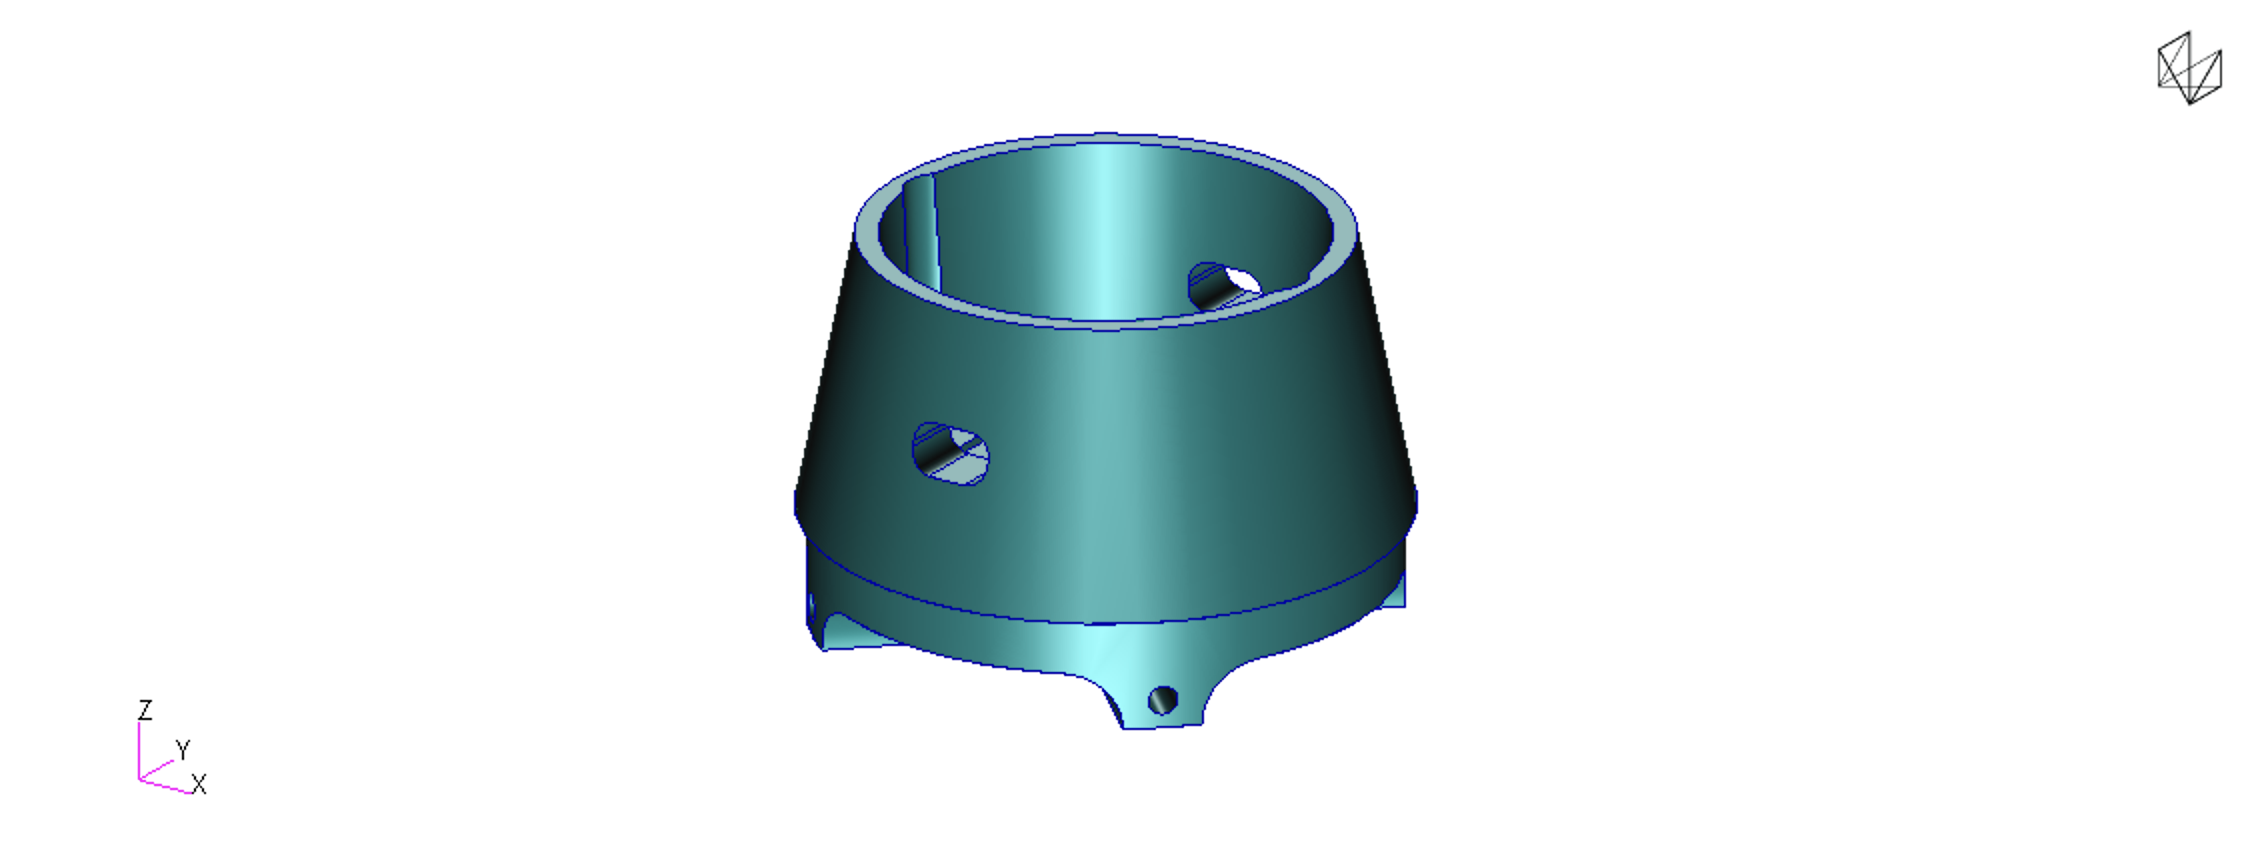
\includegraphics[width=1\linewidth]{figures/visu_import_patran.png}
	\caption{Importation de géométrie dans Patran}
     \end{figure}

    %  \notebox{Lors d'imports de pièces de CATIA à Patran, le choix de l'unité est primordial.
    %  L'unité de base est le inch (in) et doit être modifiée dans le Système International du logiciel de CAO.
    %  Ici, nous utilisons les mm.}

    \item \textbf{Maillage} :
    Le maillage est une étape fondamentale dans la caractérisation de l'étude par éléments finos.
    Toute étude doit être composée d'une analyse de convergence de maillage, c'est-à-dire
    que pour plusieurs valeurs 
    maillage trop grossier peut conduire à des résultats imprécis, tandis qu'un 
    maillage trop fin peut augmenter inutilement le temps de calcul. Dans ce projet, 
    différents types d'éléments ont été utilisés en fonction de la complexité des 
    structures :
    \begin{itemize}
        \item \textbf{Éléments 1D} : Utilisés pour modéliser des structures filiformes 
	comme les poutres ou les treillis.
        \item \textbf{Éléments 2D} : Utilisés pour les structures minces comme les 
	plaques ou les coques.
        \item \textbf{Éléments 3D} : Utilisés pour les structures volumiques complexes.
    \end{itemize}
    Des études de convergence de maillage ont été réalisées pour s'assurer que les 
    résultats sont indépendants de la taille des éléments.

    \item \textbf{Conditions aux limites} :
    Les conditions aux limites (encastrements, appuis simples, charges ponctuelles ou 
    réparties) sont définies pour reproduire les contraintes réelles subies par les 
    structures. Une attention particulière est portée à la représentation fidèle des 
    liaisons mécaniques et des charges appliquées, définies comme ceci :

    \begin{align*}
	\text{Encastrement : } 	& \begin{cases}	\text{Translations}&<0,0,0>\\ 
						\text{Rotations}&<0,0,0>  \end{cases}\\
	\text{Appui simple : } 	& \begin{cases}	\text{Translations}&<~,~,0>\\ 
						\text{Rotations}&<0,0,~>  \end{cases}\\	
	\text{Libre : } 	& \begin{cases}	\text{Translations}&<~,~ ,~ >\\ 
						\text{Rotations}&<~ ,~ ,~ > \end{cases}\\
    \end{align*}

    \item \textbf{Matériaux} :
    Les propriétés des matériaux (module de Young "E", coefficient de Poisson "$\nu$", densité "$\rho$", 
    limite élastique, couches pour matériaux composites...) sont définies suivant leur 
    comportement. Ces données influencent directement les résultats des simulations et doivent être 
    choisies avec soin pour refléter le comportement réel des matériaux. De plus, la 
    concordance des unités est une source d'erreur dans le paramétrage sur Patran. 


    \item \textbf{Analyses réalisées} :
    Plusieurs types d'analyses ont été menées, notamment :
    \begin{itemize}
        \item \textbf{Analyse statique} : Détermination des contraintes et déformations 
	sous des charges constantes. Cette analyse permet d'évaluer la résistance et la 
	rigidité des structures.
        \item \textbf{Analyse modale} : Calcul des fréquences naturelles et des modes 
	de vibration des structures. Cette analyse est essentielle pour éviter les 
	phénomènes de résonance et pour comprendre le comportement dynamique des 
	structures.
        \item \textbf{Analyse de flambement} : Évaluation de la charge critique 
	conduisant à l'instabilité des structures élancées. Cette analyse est cruciale 
	pour les structures soumises à des charges de compression.
        \item \textbf{Analyse dynamique} : Étude de la réponse des structures à des 
	sollicitations temporelles (chocs, vibrations, charges harmoniques). Cette 
	analyse permet de comprendre le comportement des structures sous des charges 
	variables dans le temps.
    \end{itemize}
\end{itemize}

\subsubsection{Méthodologie de calcul}

La méthodologie suivie pour les analyses par \acrshort{FEM} est structurée en plusieurs 
étapes clés, assurant une approche rigoureuse et systématique :

\begin{enumerate}
    \item \textbf{Préparation du modèle} :
    Cette étape inclut l'importation ou la création de la géométrie, la définition des 
    propriétés des matériaux (module de Young, coefficient de Poisson, densité, etc.), 
    et l'application des conditions aux limites (encastrements, appuis, charges). Une 
    attention particulière est portée à la représentation fidèle des détails géométriques
     et des conditions réelles de chargement.

    \item \textbf{Maillage} :
    La génération d'un maillage adapté à la géométrie et au type d'analyse est 
    essentielle. Des études de convergence de maillage sont réalisées pour s'assurer 
    que les résultats sont indépendants de la taille des éléments. Cela implique souvent 
    de raffiner le maillage dans les zones de forts gradients de contraintes (par 
    exemple, autour des trous ou des entailles).

    \item \textbf{Validation du modèle} :
    Les résultats numériques sont comparés avec des solutions analytiques ou des données
     expérimentales pour valider la pertinence du modèle. Cette étape permet de s'assurer
      que le modèle numérique représente fidèlement le comportement physique de la 
      structure.

    \item \textbf{Simulation} :
    Les calculs sont exécutés à l'aide de Nastran. Les résultats incluent les champs de 
    contraintes, de déformations, les modes de vibration, et les charges critiques de 
    flambement. Les temps de calcul peuvent varier en fonction de la complexité du 
    modèle et du type d'analyse.

    \item \textbf{Post-traitement} :
    Les résultats sont analysés via Patran pour visualiser les contraintes, les 
    déformations, et identifier les zones critiques. Des outils de post-traitement 
    permettent également d'exporter les données pour une analyse plus approfondie 
    (par exemple, traçage de graphiques dans Excel ou MATLAB).

    \item \textbf{Optimisation} :
    Sur la base des résultats, des optimisations topologiques ou géométriques sont 
    proposées pour améliorer les performances des structures. Cela peut inclure la 
    réduction de masse, l'augmentation de la rigidité, ou l'optimisation de la 
    répartition des contraintes.
\end{enumerate}

\subsubsection{Protocole de calcul analytique}

En parallèle des simulations numériques, des calculs analytiques ont été réalisés pour 
valider les résultats obtenus par \acrshort{FEM}. Ces calculs reposent sur des théories 
classiques de la mécanique des structures et permettent de fournir une référence pour 
évaluer la précision des modèles numériques.

\begin{itemize}
    \item \textbf{Théorie des poutres} :
    Utilisée pour les structures élancées soumises à des charges de flexion, torsion ou 
    compression. Les formules analytiques, comme la formule d'Euler pour le flambement, 
    permettent de calculer les contraintes et déformations maximales. Par exemple, pour 
    une poutre encastrée-libre, la charge critique de flambement est donnée par :
    \[
    P_{cr} = \frac{\pi^2 E I}{(K L)^2}
    \]
    où \(E\) est le module de Young, \(I\) le moment d'inertie, \(L\) la longueur de la 
    poutre, et \(K\) le facteur de longueur effective dépendant des conditions aux 
    limites.

    \item \textbf{Théorie des plaques et coques} :
    Appliquée pour analyser les structures minces soumises à des charges transverses 
    ou dans leur plan. Les équations différentielles régissant le comportement des 
    plaques sont résolues pour obtenir les fréquences naturelles et les modes de 
    déformation. Par exemple, pour une plaque rectangulaire simplement appuyée, les 
    fréquences naturelles sont données par :
    \[
    f_{m,n} = \frac{\pi}{2} \sqrt{\frac{D}{\rho h}} \left( \left( \frac{m}{a} \right)^2
     + \left( \frac{n}{b} \right)^2 \right)
    \]
    où \(D\) est la rigidité en flexion, \(\rho\) la densité, \(h\) l'épaisseur, et
     \(a\) et \(b\) les dimensions de la plaque.

    \item \textbf{Méthode de Rayleigh-Ritz} :
    Utilisée pour estimer les fréquences naturelles des structures en se basant sur 
    des formes modales supposées. Cette méthode permet d'obtenir des approximations 
    des fréquences naturelles sans résoudre directement les équations différentielles.

    \item \textbf{Comparaison avec la \acrshort{FEM}} :
    Les résultats analytiques servent de référence pour évaluer la précision des modèles
     numériques. Les écarts observés entre les résultats analytiques et numériques sont 
     analysés pour identifier les sources d'erreur, telles que le maillage, les conditions
      aux limites, ou les hypothèses simplificatrices.
\end{itemize}

\subsubsection{Définition des paramètres d'étude}

Pour chaque étude, les paramètres suivants ont été définis avec soin pour assurer la 
pertinence et la précision des analyses :

\begin{itemize}
    \item \textbf{Géométrie} :
    Les dimensions des structures, la position des trous, les épaisseurs, et autres
     détails géométriques sont définis avec précision. Ces détails influencent 
     directement les résultats des simulations et doivent être représentés fidèlement.

    \item \textbf{Matériaux} :
    Les propriétés mécaniques des matériaux (module de Young \(E\), coefficient de 
    Poisson \(\nu\), densité \(\rho\), limite élastique \(\sigma_y\)) sont définies en 
    fonction des spécifications du projet. Ces propriétés sont essentielles pour 
    calculer les contraintes, déformations et comportements dynamiques des structures.\\

    Le choix des matériaux a été réalisé de plusieurs manières :
    \begin{itemize}
	\item La disponibilité des matières premières sur les sites d'usinage CNC (tels l'aluminium 6061-T6, l'aluminium 7075-T6, le nylon 6,...)
	\item La disponibilité des matières premières au sein de l'association, ainsi que leur facilité d'usinage, et qui soit le moins dangemreux à manipuler et conserver.
	\item Le coût des matières brutes par rapport aux performances apportées.
    \end{itemize}
	

	Ces choix nous ont permis de confirmer l'ensemble des matériaux que ce soit pour nos tubes porteurs en fibre de verre, les
    bagues de maintien de parachute ou d'autres composants.


	\begin{table}[h!]
	\centering
	\begin{tabular}{|p{2cm}|p{1.2cm}|p{1.8cm}|p{1.8cm}|p{3cm}|p{2cm}|p{0.8cm}|}
		\hline
		Matériau & Densité (kg/m$^3$) & Module de Young (GPa) & Limite d'élasticité (MPa) & Résistance maximale en traction (MPa) & Température max. (°C) & Coût \\ \hline
		Alu 6061-T6 & 2700 & 69 & 276 & 310 & 150 & €€ \\ \hline
		Alu 7075-T6 & 2810 & 71 & 503 & 572 & 150 & €€€ \\ \hline
		Acier (304) & 8000 & 193 & 240 & 620 & 650 & €€€€ \\ \hline
		Laiton & 8530 & 105 & 300 & 450 & 200 & €€ \\ \hline
		GFRP (163 g/m$^2$) & 1850 & 25 & — & 500 & 150 & €€€ \\ \hline
		PETG & 1280 & 1,81 (x-y) / 1,54 (z) & 50--55 & 55--60 (x-y) / 35--40 (z) & 80--90 & € \\ \hline
		POM-C & 1410 & 2,8--3,2 & 60--70 & 65--75 & 100--110 & €€ \\ \hline
		Nylon 6 & 1140 & 2,5 & 70 & 80 & 120 & €€ \\ \hline
	\end{tabular}
	\caption{Propriétés mécaniques et coût des matériaux sélectionnés}
	\label{tab:choix_materiaux}
	\end{table}



\newpage
    \item \textbf{Charges appliquées} :
    La nature (ponctuelle, répartie, harmonique), l'amplitude et la direction des 
    charges sont définies pour reproduire les conditions réelles de chargement. Par 
    exemple, une charge harmonique peut être définie par :
    \[
    F(t) = F_{\text{max}} \sin(2 \pi f t)
    \]
    où \(F_{\text{max}}\) est l'amplitude maximale de la charge et \(f\) la fréquence.

    \item \textbf{Conditions aux limites} :
    Le type de liaisons (encastrement, appui simple, libre) et leur localisation sont 
    définis pour représenter les contraintes réelles subies par les structures. Par 
    exemple, un encastrement parfait empêche tout déplacement et rotation, tandis qu'un 
    appui simple permet la rotation mais pas le déplacement.

    \item \textbf{Critères de validation} :
    Les tolérances acceptables pour les écarts entre les résultats analytiques et 
    numériques sont généralement fixées à moins de 5\% pour les fréquences naturelles 
    et les contraintes maximales. Ces critères permettent de valider la précision des 
    modèles numériques.
\end{itemize}



\subsubsection{Limites}

Malgré sa puissance et sa polyvalence, la méthode des éléments finis (\acrshort{FEM}) 
présente certaines limites qui doivent être prises en compte pour une interprétation 
correcte des résultats :

\begin{itemize}
    \item \textbf{Hypothèses simplificatrices} :
    Les modèles numériques reposent sur des hypothèses qui peuvent ne pas refléter 
    parfaitement la réalité. Par exemple, les analyses linéaires supposent un 
    comportement élastique des matériaux et de petites déformations, ce qui peut ne pas 
    être le cas pour des charges élevées ou des matériaux non linéaires.

    \item \textbf{Maillage} :
    La qualité des résultats dépend fortement de la finesse du maillage. Un maillage 
    inadapté peut conduire à des erreurs significatives, en particulier pour les 
    structures présentant des gradients de contraintes élevés (par exemple, autour des 
    trous ou des entailles). Des études de convergence de maillage sont donc essentielles
     pour s'assurer de la précision des résultats.

    \item \textbf{Conditions aux limites} :
    Les conditions aux limites modélisées dans Patran sont souvent des idéalisations 
    des conditions réelles. Par exemple, un encastrement parfait dans un modèle 
    numérique peut ne pas représenter fidèlement une liaison boulonnée ou soudée dans 
    la réalité, ce qui peut introduire des écarts dans les résultats.

    \item \textbf{Temps de calcul} :
    Les analyses complexes, telles que les analyses dynamiques transitoires ou 
    non-linéaires, peuvent nécessiter des ressources informatiques importantes et 
    des temps de calcul longs. Cela peut limiter la taille des modèles ou la finesse 
    du maillage pour des projets avec des contraintes de temps.

    \item \textbf{Validation expérimentale} :
    Bien que les résultats numériques soient cohérents avec les calculs analytiques,
    une validation expérimentale reste essentielle pour confirmer leur pertinence, 
    notamment pour les structures soumises à des charges dynamiques ou cycliques. Les 
    essais expérimentaux permettent de valider les hypothèses et les résultats des 
    simulations numériques.
\end{itemize}

\subsection{Validation des pièces concues (contraintes du cahier des charges)}
Avec pour perspective, la fabrication réelle des pièces modélisées et simulées par 
éléments fins, l'ensemble des pièces de notre lanceur doit être approuvé par le cahier 
des charges (CDC) \gls{Fusex} ainsi qu'à des règles supplémentaires. Parmi ces
 règles, nous pouvosn citer la tenue mécanique lors des phases de vol, le double empennage, 
la flèche, le bon dimensionnement des parachutes... \\
Ce tableau ci-dessous récapitule les règles de structure globale détaillées dans le 
\acrshort{CDC} afin de définir les forces d'applications et conditions aux limites.
l'ensemble de nos matériaux pour les composants soumis à de fortes contraintes.

\begin{table}[h!]
\centering
\begin{tabular}{|p{1.2cm}|p{4cm}|p{10cm}|}
\hline
Règles & Type & Détails du cahier des charges \\ \hline

MEC1  & Flèche & Les flèches statiques de l’étage 2 et de l’ensemble doivent être inférieures ou égales à 1\% (10 mm/m) \\ \hline
MEC2  & Tenue en compression & Chaque élément de l’étage 2 et de l’ensemble doit pouvoir supporter une compression équivalente à F = 2 x Accélération Max x Msup (en N) \\ \hline
MEC3  & Résistance longitudinale des ailerons & Les ailerons doivent pouvoir supporter une force longitudinale de : F = (2 x Masse d’un aileron x Accélération Max) + (0,02 x Surface d’un aileron x Vmax² x Coefficient de traînée) \\ \hline
MEC4  & Résistance transversale des ailerons & Une force F = 0,1 x Surface d’un aileron x Vmax$^2$ (en NEWTON) doit entraîner une flèche transversale des ailerons inférieure à 10° \\ \hline
MEC5  & Alignement des ailerons & Alignements des ailerons par rapport à l’axe longitudinal de la fusée < 1° \\ \hline
MEC6  & Angle entre deux ailerons & Angle entre deux ailerons consécutifs : 90° ± 10° (fusex à 4 ailerons) ou 120° ± 10° (fusex à 3 ailerons) \\ \hline
MEC7  & Tenue en traction & L’étage 2 et l’ensemble doivent rester intègres quand ils sont soulevés verticalement par l'ogive les ailerons vers le bas et par les ailerons l'ogive vers le bas \\ \hline
MEC8  & Double jeu d'ailerons & Dans le cas d’une fusée à deux jeux d’ailerons, les deux jeux d’ailerons sont soumis aux règles MEC3, 4, 5 et 6 \\ \hline
MEC9  & Tenue mécanique globale & La tenue mécanique de tous les éléments de la fusée doit leur permettre de fonctionner correctement lorsqu’ils sont soumis aux perturbations du vol (accélérations, vibrations, ...) \\ \hline

\end{tabular}
\caption{Règles de structure mécanique globale issues du \acrshort{CDC} \gls{Fusex} \cite[p.~32-33]{CDC_BiEtage}}
\end{table}

\newpage